\documentclass[twocolumn]{report}

\usepackage[toc,page]{appendix}
\usepackage{amsmath, amsfonts, amssymb, amsthm}
\usepackage{tikz}
\renewcommand\thesection{\arabic{section}}
\allowdisplaybreaks
\newtheorem{definition}{Definition}
\newtheorem{theorem}{Theorem}
\newtheorem{observation}{Observation}

\newcommand\cone[1]{\textrm{cone}(#1)}
\newcommand\conv[1]{\textrm{conv}(#1)}
\newcommand\R{\mathbb R}
\newcommand\N{\mathbb N}
\newcommand\Z{\mathbb Z}

\title{Optimization Handbook}
\author{Henri Lefebvre}

\begin{document}
    \maketitle
    \tableofcontents

    \part{Linear Optimization}
    \chapter{Introduction to linear programming}

\section{Problems description}

\subsection{Definitions}
Linear programming (LP) takes interests in problems in which both the objective function and the constraints are linear with respect to the decision variables. The feasible region is therefore composed of linear inequalities or linear equalities. For the sake of generality, we often consider a problem of minimizing a linear objective function subject to equality constraints. Such a problem is said to be in \textit{standard form}. Note that the standard form is only used as a way to present a homogeneous framework for theoretical work. In the following section, we show how any formulated linear program can be reduced to a problem written in standard form.

Some examples of problems which can be formulated in a linear fashion are presented in section \ref{sec:lpb_examples}. Yet, we give here a very simple example for the sake of understanding. This problem will also allow us to have a first geometrical interpretation of some mathematical objects considered in linear programming. 

Let us consider a production plant where two kinds of items are to be produced. Both items are made of two raw matrials $RM_1$ and $RM_2$. Items of type $A$ need $10$ units of $RM_1$ and $4$ units of $RM_2$ while items of type $B$ need $2$ units of $RM_1$ and $4$ units of $RM_2$ to be produced. The problem is to decide how many items of type $A$ and of type $B$ should be produced in the plant, knowing that the raw materials are of fixed amount. Let us assume that we have $50$ units of raw material $RM_1$ and $60$ units of $RM_2$. A so-called \textit{feasible solution} is a decision which satisfies the capacity constraints of the raw materials (i.e., we do not produce more items than we have raw material to do so). A feasible solution is said to be \textit{optimal} if it minimizes or maximizes a certain quantity. Here, we will consider the minimization of the cost. Let us assume that items of type $A$ cost $5$ euros to be produced and that items $B$ cost $4$ euros. The problem can be stated as : 
\begin{align*}
    \textrm{minimize } & 3x + 4y\\
    \textrm{s.t. } & 10x + 4y \le 50\\
    & 2x + 3y \le 30\\
    & x\ge 0, y\ge 0
\end{align*}
Here, one may argue that the decisions variables $x$ and $y$ need to take integer values. This in fact depends on the context and application of the problem. We will see however that integer linear programming (ILP) problems as well as mixed integer linear programming (MILP) where we have both continuous and integer decision variables are much harder to solve. Yet we will consider quite efficient algorithms to solve such kinds of problems, among which : the branch-and-bound approach and the cutting planes algorithm. 

Since our problem is a two-dimensional problem, in that sense that we have two decision real (or integer) variables to decide, one can plot the \textit{feasible region} of the problem. The feasible region denots the set of feasible solutions. Figure \ref{fig:feasible_region} depicts the feasible region of our problem. 

\begin{figure}[h!]
    \centering
    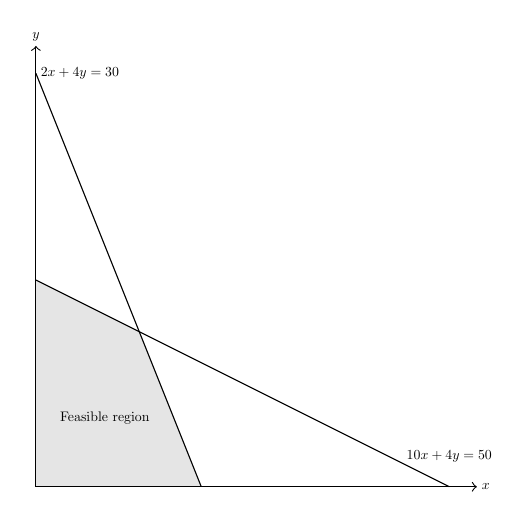
\begin{tikzpicture}[scale=.35, every node/.style={scale=.5}]
        \fill[gray!20] (0,0) -- (0,7.5) -- (3.75, 5.625) -- (6,0);
        \draw[<->] (0,16) node[above] {$y$} |- (16,0) node[right] {$x$};
        \draw (0,7.5) -- (15,0) node[above=.5cm] {$10x+4y = 50$};
        \draw (0,15) node[right] {$2x+4y = 30$} -- (6,0);
        \draw (2.5,2.5) node {Feasible region};
    \end{tikzpicture}
    \caption{2D representation of a feasible region}
    \label{fig:feasible_region}
\end{figure}

One should indeed see that above this feasible region stands a plane (or hyperplane in higher dimensions) defining the objective function. Since the objective function is a place, it is clear that the optimal solution can be found in one of the extreme points of the feasible region. This property, in fact, holds in general and is called the \textit{Fundamental theorem of linear programming} and will be formally introduced in section \ref{sec:fonda_th}. 

\subsection{Standard form}

\subsubsection{Formal definition}

% As previously introduced, we give here the formal definition of the standard form for LP problems :

\begin{definition}[Standard form]
    A linear programming problem is said to be in standard form if it is written as
    \begin{align*}
        \textrm{minimize } & c^Tx \\
        \textrm{s.t. } & Ax = b\\
        & x\ge 0
    \end{align*}
\end{definition}

\subsubsection{Examples}

In this section, we show how we can turn linear problems which are not originally in the standard form to a problem written in standard form.

\paragraph{Negative variables}
If a given problem uses a negative variable, say $x\le 0$. It suffices to consider the opposite decision variable $\hat x = -x$. The problem is now in standard form. 

\paragraph{Real variables}
If a given problem uses a free variable (i.e., a variable which can be positive or negative) $x\in\R$. We introduce two positive decision variables $x^+\ge 0$ and $x^-\ge 0$ and write $x$ as $x^+ - x^- \in\R$. The problem is now in standard form. 

\paragraph{Inequality constraints}
If a given problem defines the feasible region with inequality constraint, so-called \textit{slack} variables can be introduced. Considering an inequality constraint $\sum_j a_jx_j \le b$, we introduce variable $s\ge 0$ so that $\sum_j a_jx_j + s = b$. We do not restrict the values of $s$ (other than by its sign) and do not associate any cost in the objective function. Therefore, the value of $s$ in the optimal solution corresponds to the $b-\sum_j a_jx_j$, hence the name of slack variables. The obtained problem is now in standard form. 

\section{Fundamental Theorem of LP}
\label{sec:fonda_th}

The fundamental theorem of linear programming as been intuitively introduced in the previous section. We enounce it here formally and prove its validity and geometrical interpretation. First, we introduce the following assumption which will hold in general in the subsequent theorems :

\begin{assumption}[Full rank assumption]
    \label{ass:full_rank}
    Considering the feasible region $\{x|Ax = b, x\ge 0\}$ where $A$ is a $m\times n$ matrix. We assume that $\rank{A}=n$
\end{assumption}

The fundamental theorem of LP characterizes the optimal solutions of a given problem. In that sense, it reduces the search space for optimality. To properly enouce the theorem, we need to introduce the concept of \textit{basic} solutions.

Consider a feasible region defined as \[ \{ x\in\R | Ax = b, x\ge 0 \} \] where $A$ is a $m\times n$-matrix of full rank (see assumption \ref{ass:full_rank}). If we select $n$ linearly independent columns from $A$, then the set of columns represent a basis of $\R^n$. Let us denote by $B$ the matrix corresponding to that basis. Since $B$ is non-singular, the following system can be solved uniquely :
\[ Bx_B = b \] where $x_B$ is an $m$-dimensional vector. Then, clearly, the vector $x$ defined as $x = [x_B, \textbf 0]$ belongs to the feasible region since $Ax = A[x_B, \textbf 0] = Ax_B + A\textbf 0 = b$. This consideration leads to the following definition :

\begin{definition}[Basic solution]
    Considering a feasible region $\{x\in\R|Ax=n,x\ge 0\}$ where $A$ is a matrix of full rank.
    A vector $x$ is said to be basic if and only if there exists a basis $B$ of $\R^n$ composed of $n$ columns of $A$ and $x = [B^{-1}b, \textbf 0]$. If, moreover, it is positive element-wise then it is said to be a feasible basic solution. 
\end{definition}

We can now enounce the theorem :

\begin{theorem}[Fundamental theorem of linear programming]
    \label{th:fundamental}
    Consider the following LP problem in standard form :
    \begin{align*}
        \textrm{minimize } & c^Tx\\
        \textrm{s.t. } & Ax = b\\
        & x \ge 0
    \end{align*}
    Then, under the full rank assumption (\ref{ass:full_rank}),
    \begin{enumerate}[label=(\roman*)]
        \item if there is a feasible solution, there is a basic feasible solution
        \item if there is an optimal feasible solution, there is an optimal basic feasible solution.
    \end{enumerate}
\end{theorem}
\begin{proof}\leavevmode
    \begin{enumerate}[label=(\roman*)]
        \item Let $x$ be a feasible solution and let us denote by $a_1,...,a_n$ the columns of $A$. Since it is feasible, the following holds : \[ a_1x_1 + ... + a_nx_n = b \] Assume now that exactely $p$ variables $x_i$ are greater than zero. For the sake of exposure, we'll assume that they correspond to the $p$ first variables. That is : \[ a_1x_1 + ... + a_px_p = b \] Then two different situations may occur : 
        \begin{description}
            \item[$(a_1,...,a_p)$ are linearly independent] : then clearly we have $p\le m$. If $p=m$, then $x$ is a basic feasible solution and the proof is complete. If $p<m$ then since $A$ is of full rank, one can find $m-p$ columns of $A$ which forms a basis when added to the $p$ columns $a_1,...,a_p$. By setting $x_i = 0$ for all $i>p$, we obtain a (degenerate) basic feasible solution. 
            \item[$(a_1,...,a_p)$ are linearly dependent] :
            Then there exists coefficients $\lambda_i,...,\lambda_p$ all non-zero, at least one of which can be assumed to be positive, such that \[ a_1\lambda_1 + ... + a_p\lambda_p = 0 \] Let $\varepsilon\in\R$, Since $Ax = b$ holds, it also holds that \begin{equation} (x_1 - \varepsilon\lambda_1)a_1 + ... + (x_p-\varepsilon\lambda_p)a_p = b \label{eq:built_solution} \end{equation} For $\varepsilon = 0$, this reduces to the original feasible solution. As $\varepsilon$ increases, the different components may increase, decrease or remain constant depending on the sign of $\lambda_i$. Since we assumed that at least one $\lambda_i$ is positive, then at least one component will decrease as $\varepsilon$ increases. We increase $\varepsilon$ to the first point where one or more components become zero. That is, we choose \[ \varepsilon = \min\{ x_i/\lambda_i : \lambda_i > 0 \} \] For this specific value, the solution built in \ref{eq:built_solution} is feasible and has at most $p-1$ positive variables. Repeating this process as much as necessary, we can eliminate positive variables untill we obtain a feasible solution with corresponding columns which are linearly dependent. 
        \end{description}
        \item Let us consider an optimal solution $x^*$ and, as in proof of $(i)$, let us suppose that there are exactely $p$ positive variables. Again, two cases may occure as to whether the selected columns of $A$ are linearly dependent or not. If the columns are independent, the proof goes as for $(i)$. If they are dependent, we still can apply the idea of the proof of $(ii)$ yet we need to check that the objective value of $x^* - \varepsilon \lambda$ remains optimal. Note that the objective value of the constructed solution is \[ c^Tx^* + \varepsilon c^T\lambda \] By contradiction, suppose that $c^T\lambda\ne 0$. Then one can find a sufficiently small value for $\varepsilon$ so that $c^Tx^* + \varepsilon c^T\lambda < c^Tx^*$ which contradicts the optimality of $x^*$. Hence, $c^Ty = 0$ and the obtained solution is optimal. 
    \end{enumerate}
\end{proof}

Before stating an equivalence result previously mentioned between basic variables and extreme points of polyhedra, let us take a small detour with a geometrical example of the idea of the proof of theorem \ref{th:fundamental}, point \textit{(i)}. For that purpose, let us consider the following feasible region : \[ K = \left\{ x\in\R^3_+ \middle| \begin{array}{ll} x_1 + x_2 + x_3 &= 1 \\ x_2 + x_3 &= \frac 23 \end{array} \right\} \] $K$ is depicted in figure \ref{fig:3d_feasible}. As well, a (non-basic) feasible point is depicted with coordinates $(\frac 13, \frac 13, \frac 13)$. Indeed, one can easily check that \[ \frac 13 \begin{pmatrix} 1\\ 1 \end{pmatrix} + \frac 13 \begin{pmatrix} 1\\ 0 \end{pmatrix} + \frac 13 \begin{pmatrix} 1\\1 \end{pmatrix} = \begin{pmatrix} 1\\\frac 23 \end{pmatrix} \] Yet, clearly, this collection of vectors are linear dependent, in particular we have : \[ 1 \begin{pmatrix} 1\\ 1 \end{pmatrix} + 0 \begin{pmatrix} 1\\ 0 \end{pmatrix} + (-1) \begin{pmatrix} 1\\1 \end{pmatrix} = \begin{pmatrix} 0\\ 0 \end{pmatrix} \] From the two above equations, we obtain by multiplying the second one by a scalar $\varepsilon>0$ and subtracting the first one : \[ \left(\frac 13 - \varepsilon\right) \begin{pmatrix} 1\\ 1 \end{pmatrix} + \frac 13 \begin{pmatrix} 1\\ 0 \end{pmatrix} + \left(\frac 13 + \varepsilon\right) \begin{pmatrix} 1\\1 \end{pmatrix} = \begin{pmatrix} 1\\\frac 23 \end{pmatrix} \] If we choose $\varepsilon = \frac 13$ (i.e., $\min\{ x_i/\lambda_i : \lambda_i > 0 \}$), we find that $x = (0,\frac 23, \frac 13)$ is also a feasible solution and it has one coefficient set to zero. Since we have two constraints ($m=2$), this solution is a basic solution (also depicted in figure \ref{fig:3d_feasible}).

\begin{figure}[h!]
    \centering
    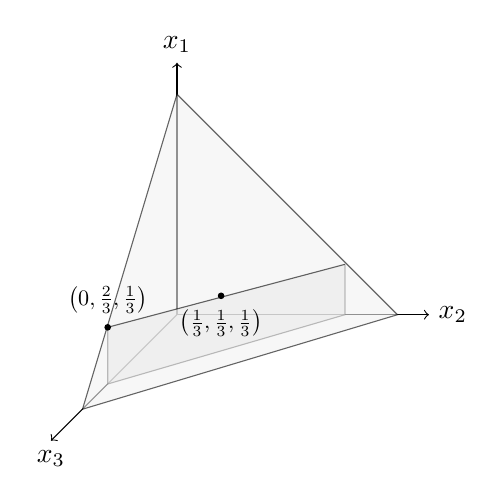
\begin{tikzpicture}[scale=.8]
        \draw[<->] (0, 4) node[above] {$x_1$} |- (4, 0) node[right] {$x_2$};
        \draw[->] (0,0) -- (-2, -2) node[below] {$x_3$};
        \draw[fill=gray!25, opacity=.6] (8/3,.8) -- (4*2/3,0) -- (-1.1,-1.1) -- (-1.1,-.2);
        \draw[fill=gray!10, opacity=.6] (-1.5,-1.5) -- (0,3.5) -- (3.5,0) -- cycle;
        \draw[opacity=.6] (8/3,.8) -- (-1.1,-.2);
        \fill[black] (.7,.3) circle (1.5pt) node[scale=.8, below=.1cm] {$\left(\frac 13,\frac 13,\frac 13\right)$};
        \fill[black] (-1.1,-.2) circle (1.5pt) node[scale=.8, above=.1cm] {$\left(0,\frac 23, \frac 13\right)$};
    \end{tikzpicture}
    \caption{3D representation of feasible region $K$}
    \label{fig:3d_feasible}
\end{figure}

We can see that our basic feasible solution is indeed an extreme point of the polytope $K$. The following theorem states that this remark holds in general. 

\begin{theorem}[Equivalence between basic solutions and extreme points]
    Considering a matrix $A$ of full rank (see assumption \ref{ass:full_rank}), a vector $x$ is an extreme point of the polyhedron $\{x|Ax=b, x\ge 0\}$ if and only if it is a basic feasible solution.
\end{theorem}
\begin{proof}\leavevmode
    \begin{description}
        \item[$\Rightarrow$] : Let $x$ be a basic feasible solution for $\{ x | Ax = b, x\le 0 \}$ where $A$ is a $m\times n$ matrix. We have \[ a_1x_1 + ... + a_mx_m = b \] By contradiction, let us suppose that there exists two different points $y,z\in\{x|Ax=b,x\ge 0\}$ such that $x$ is a convex combination of these points, i.e., : \[ x = \alpha y + (1 - \alpha) z \quad 0<\alpha<1 \] Since $x\ge 0$ and $\alpha$ is positive, it holds that the last $n-m$ components of $y$ and $z$ are also equal to zero. Thus :
        \begin{align*} 
            y_1a_1 + ... + y_ma_m = b\\
            z_1a_1 + ... + z_ma_m = b
        \end{align*} Yet since $a_1,...,a_m$ are linearly independent, it follows that $x=y=z$ which contradicts that $y\ne z$. Hence, $x$ is an extreme point.
        \item[$\Leftarrow$] : Let $x$ be an extreme point of $\{ x | Ax = b, x\ge 0 \}$ and let us assume that the nonzero components of $x$ are the first $k$ components, i.e., \[ a_1x_1 + .... + a_kx_k = b \] Let us show that $a_1,...,a_k$ are linearly independent (i.e., that $x$ is a basic feasible solution). By contradiction, suppose that $a_1,...,a_k$ are linearly dependent. Then, there exists a vector $\lambda \ge 0$ with at least one non-zero coefficient such that \[ \lambda_1a_1 + ... + \lambda_ka_k = 0 \] Since $x\ge 0$, one can find a value for $\varepsilon$ such that \[ x + \varepsilon\lambda\ge 0\quad x-\varepsilon\lambda \ge 0 \] Yet, if this were the case, it would holds that $x = \frac 12 (x + \varepsilon\lambda) + \frac 12(x-\varepsilon\lambda)$ which is a convex combination of two distinct feasible points. This contradicts the fact that $x$ is an exterme point. Hence, $x$ is a basic feasible solution. 
    \end{description}
\end{proof}

One final remark should be made regarding the definition of a basic solution. Indeed, in general, the coefficients of a basic solution may not be all non-zero. We therfore give the following definition :
\begin{definition}[Degenerate solution]
    A basic solution is said to be degenerate if and only if one or more of the basic variables value are zero.
\end{definition}
Note that, in presence of degeneracy, ambiguity arises since one could interchange freely the zero-valuated basic variables with non-basic variables.

\begin{observation}
    The fundamental theorem of linear programming reduces the search space for optimality to the set of extreme points of the feasible region. Yet, note that for a problem with $n$ variables and $m$ constraints, we have at most \[ \begin{pmatrix} n\\ m \end{pmatrix} = \frac{n!}{m!(n-m)!} \] extreme points (or equivalently, basic solutions). 
\end{observation}

\section{Examples}
\label{sec:lpb_examples}
\subsection{Minimum cost flow problem}
\subsection{Support Vector Machine}
\subsection{Knapsack problem}

    \chapter{Lagrangian duality}

\section{Motivations}

\section{Practical derivations}

\section{Duality theorems}

\section{Geometric interpretation}

\section{Sensitivity}

\section{Complentary slackness}

\section{The Primal-Dual algorithm}

\subsection{Examples}

    \chapter{The Simplex algorithm}

\section{Formal derivation}

\subsection{Assumptions}
\begin{assumption}[Nondegeneracy assumption]
    Every basic feasible solution is a nondegenerate basic
feasible solution.
\end{assumption}

\subsection{Vector leaving the basis}

\subsection{Vector entering the basis}

\section{Geometrical Interpretation}

\section{Finding a feasible solution}

\section{The Simplex method}

\subsection{Pseudo-code}
\subsection{Degeneracy}
\subsection{Examples}
\subsubsection{Optimal solution}
\subsubsection{Degenerate solution}
\subsubsection{Unbounded problem}
\subsubsection{Infeasible problem}

\section{The revised Simplex}
\subsection{Matrix form of the Simplex}
\subsection{Pseufo-code}
\subsection{Examples}

\section{The bounded Simplex}
\subsection{Formal derivation}
\subsection{Pseudo-code}
\subsection{Examples}

\section{The transportation Simplex}
\subsection{Formal derivation}
\subsection{Pseudo-code}
\subsection{Examples}

    \chapter{Relaxation techniques}

\section{Formal definition}

\section{Linear relaxation}

\section{Lagrangian relaxation}

\section{Surrogate relaxation}
    \chapter{The branch-and-bound algorithm}
    \chapter{The branch-and-cut algorithm}
    \chapter{Column generation and the branch-and-price algorithm}
    \chapter{Benders decomposition}

\section{Introduction}

Benders decomposition is a solution method for solving certain large-scale optimization problems. It is particularly suited for problems in which a set of variables are said to be \textit{complicating} in the sense that fixing them to a given value makes the problem easy. Briefly, the Benders decomposition approach seperates an original problem into several decision stages. A first-stage \textit{master} problem is solved using only a subset of variables, then, the values of the remaining variables are determined by a so-called \textit{subproblem} depending on the first-stage variables. If the master problem's optimal solution yields an infeasible subproblem, a \textit{feasibility cut} is added to the master problem, which is then re-solved. Due to the structure of the reformulation, the Benders algorithm starts with a \textit{restricted master problem} where only a subset of constraints are considered while the others are iteratively added. 

This technique was first introduced in \cite{Benders1962} and has since been generalized to non-linear mixed integer problems. 

\section{Formal derivation}

Consider the following problem :
\begin{align}
    \textrm{minimize } & c^Tx + f(y) \\
    \textrm{s.t. } & Ax + g(y) = b \\
    & y\in Y, x\ge 0
\end{align} where variable $y$ is a \textit{complicating constraint}. Note that it may be complicating due to the form of $f$ or $g$ but also by our ability to enforce the constraint $y\in Y$. We assume that fixing $y$ to a given value $\hat y$ turns our problem into an easy-to-solve problem. 

We can notice that our problem is equivalent to the following one : \[
    \min\left\{ f(y) + \min\left\{ c^Tx : Ax = b - g(y) \right\} : y \in Y \right\}
\] Let us denote by $q(y)$ the value of the minimization problem over $x$ : $q(y) = \min\{ c^Tx : Ax = b - g(y) \}$. By duality, the following holds \[
    q(y) = \max\{ (b-g(y))^T\pi : A^T\pi \le c \}
\]
    \input{parts/linear/dantzig-wolfe.tex}

    \part{Non-linear Optimization}

    \begin{appendices}
        \chapter{Convexity}

\begin{definition}[Minkowski sum]
    Let $A$ and $B$ be two vector spaces, the Minkowki sum is defined as
    \[
        A + B = \{ a + b | a\in A, b\in B \}
    \]
\end{definition}

\begin{definition}[Convex combination]
    Let $x_1,...,x_n$ be a finite set of vectors in a real vector space, a convex combination of these vectors is a vector of the form 
    \[
        \sum_{i=1}^n\alpha_ix_i\qquad\textrm{with } \sum_{i=1}^k\alpha_i = 1, \alpha\ge 0
    \]
\end{definition}

\begin{definition}[Convex hull]
    \[
        \conv{X} = \left\{ \sum_{i=1}^n\alpha_ix_i \middle| x_i\in X, \sum_{i=1}^n\alpha_i = 1, \alpha\ge 0 \right\}
    \]
\end{definition}

\begin{definition}[Conical combination]
    Let $x_1,...,x_n$ be a finite set of vectors in a real vector space, a conical combination of these vectors is a vector of the form 
    \[
        \sum_{i=1}^k \alpha_ix_i \qquad\textrm{with } \alpha\ge 0
    \]
\end{definition}

\begin{definition}[Conical hull]
\[
    \cone{X} = \left\{ \sum_{i=1}^n \alpha_ix_i \middle| x_i\in X, \alpha_i \ge 0 \right \}
\]
\end{definition}

\begin{theorem}[Affine Minkowski-Weyl]
    Let there be a polytope defined by a set of inequalities, $P = \{ x\in\R^n | Ax\le b \}$. There exists vectors $x_1,...,x_q\in\R^,n$ and $y_1,...,y_r\in\R^n$ such that
    \[
        P = \cone{x_1,...,x_q} + \conv{y_1,...,y_r}
    \]
\end{theorem}

\begin{observation}
    In the affine Minkowki-Weyl theorem, the smallest set of vectors $x_1,...,x_q$ is the set of extreme rays of $P$ and the smallest set of vectors $y_1,...,y_r$ is the set of extreme points of $P$. 
\end{observation}
    \end{appendices}

    \bibliographystyle{abbrv}
    \bibliography{references} 
\end{document}